%2586
\newpage
\subsection{例題4-12 センサーボードの入力を使ってみよう}


\begin{description}
    \item \textgt{\bf 考え方}
\end{description}

キーボードの代わりにセンサーボードのボタンを使って絵を動かしてみましょう。

move.hspのプログラムを改造して、センサーボードのボタンで絵を動かせるようにしましょう。

\begin{figure}[H]
    \begin{center}
      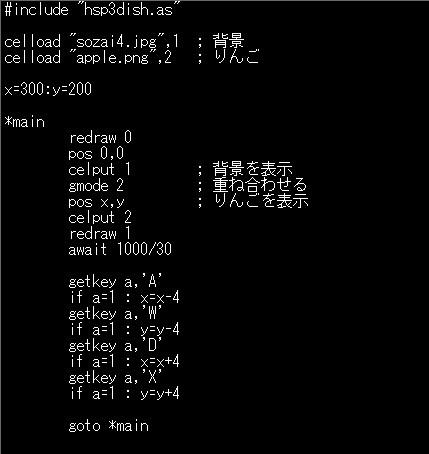
\includegraphics[keepaspectratio,width=10.61cm,height=11.229cm]{text04-img/s_move.png}
    \end{center}
    \label{fig:prog_menu}
\end{figure}

\begin{description}
    \item \textgt{\bf 例題4-12 答え}
\end{description}

以前に取り上げた、GPIOの番号とその役割を思い出してみてください。


\begin{figure}[H]
    \begin{center}
      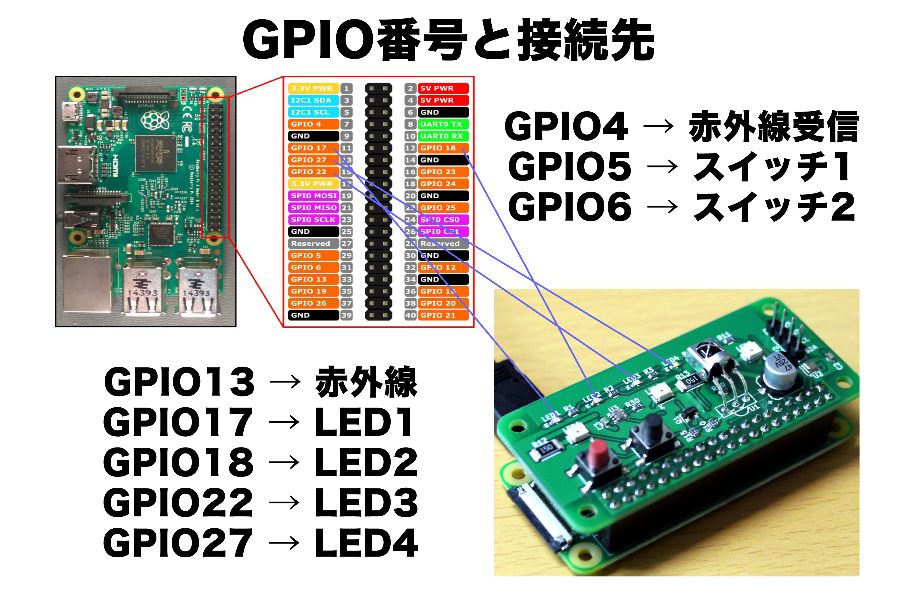
\includegraphics[keepaspectratio,width=10.372cm,height=6.89cm]{text04-img/s_gpio.png}
    \end{center}
    \label{fig:prog_menu}
\end{figure}

スイッチの状態などを知る場合は、gpioinという関数を使います。

\begin{description}
    \item \textgt{\bf \ \ 変数 = gpioin(GPIO番号)}
\end{description}

と書くことで、指定されたGPIO番号のスイッチがONかOFFかを調べることができます。

変数には0か1の数字が代入されるので、条件判断を行うif命令で違う動作をさせることができます。


\begin{description}
    \item \textgt{\bf \ \ a = gpioin(5)}
    \item \textgt{\bf \ \ if a=0 : x=x-4}
\end{description}

のように書くことで、変数aが0の時だけ「x=x-4」を実行させることができます。


以下のようにプログラムを改造することで、センサーボードのボタンを条件判断で使うことができます。

\begin{figure}[H]
    \begin{center}
      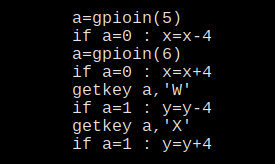
\includegraphics[keepaspectratio]{text04-img/s_gpioinif.png}
    \end{center}
    \label{fig:prog_menu}
\end{figure}

改造ができたらTAや周りの友達にも見せてあげましょう。


以前に\ruby{乱数}{らん|すう}の使い方を学習したことを思い出してみましょう。

「x=rnd(640)」は、0〜639(640通り)までのバラバラな数字を変数xに代入します。

このような書き方を「\ruby{乱数}{らん|すう}」と呼んでいます。

\begin{figure}[H]
    \begin{center}
      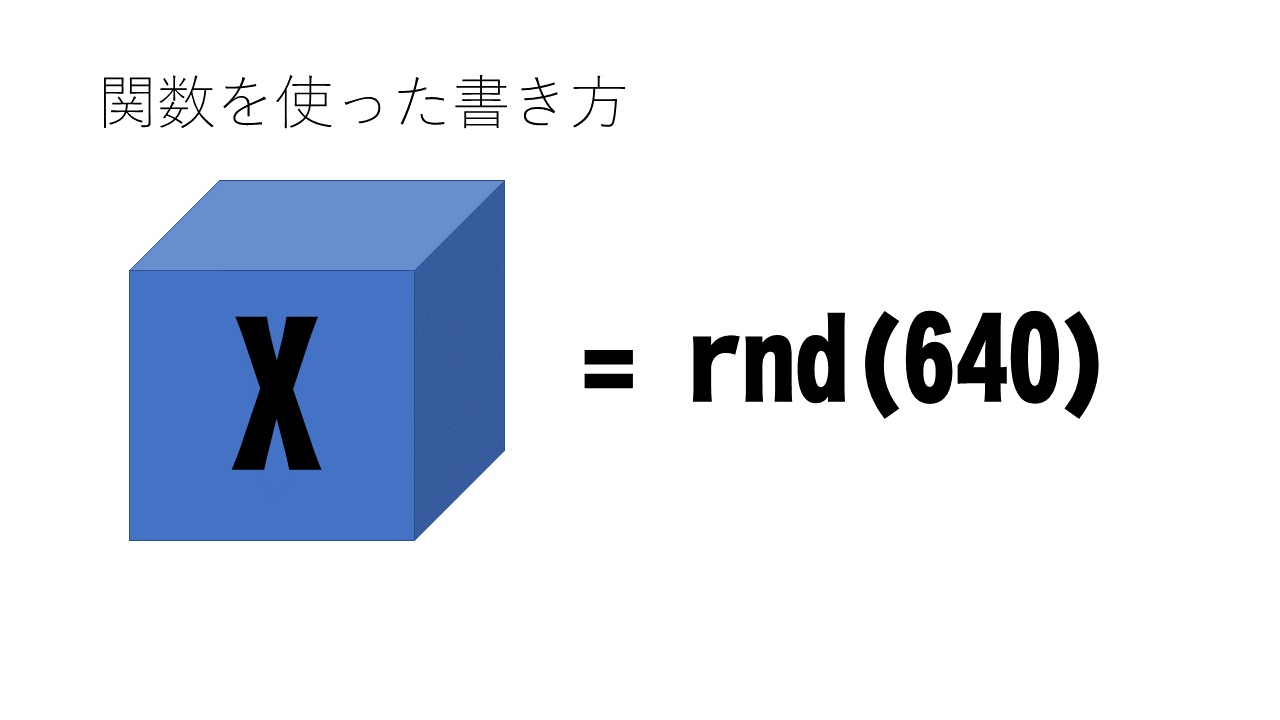
\includegraphics[keepaspectratio,width=11.906cm,height=5.662cm]{text04-img/s_rnd.png}
    \end{center}
    \label{fig:prog_menu}
\end{figure}

\begin{description}
    \item \textgt{\bf \ \ (HSPのルール)}
    \item \textgt{\bf \ \ 「変数=rnd(乱数の最大値)」でバラバラな数字を得ることができる}
    \item \textgt{\bf \ \ 関数は、「変数=関数(パラメーター)」という書き方で使うことができる}
\end{description}

乱数が代入された変数を条件判断することで、でたらめな動きをする絵を作ることもできます。

余裕がある人は、乱数を使った動きにも挑戦してみましょう。

%2720